\documentclass{article}
\usepackage{tikz}
\usetikzlibrary{shapes.geometric, arrows}

\tikzstyle{startstop} = [rectangle, rounded corners, minimum width=3cm, minimum height=1cm,text centered, draw=black, fill=red!30]
\tikzstyle{process} = [rectangle, minimum width=3cm, minimum height=1cm, text centered, draw=black, fill=blue!30]
\tikzstyle{decision} = [diamond, minimum width=3cm, minimum height=1cm, text centered, draw=black, fill=green!30]
\tikzstyle{arrow} = [thick,->,>=stealth]

\begin{document}
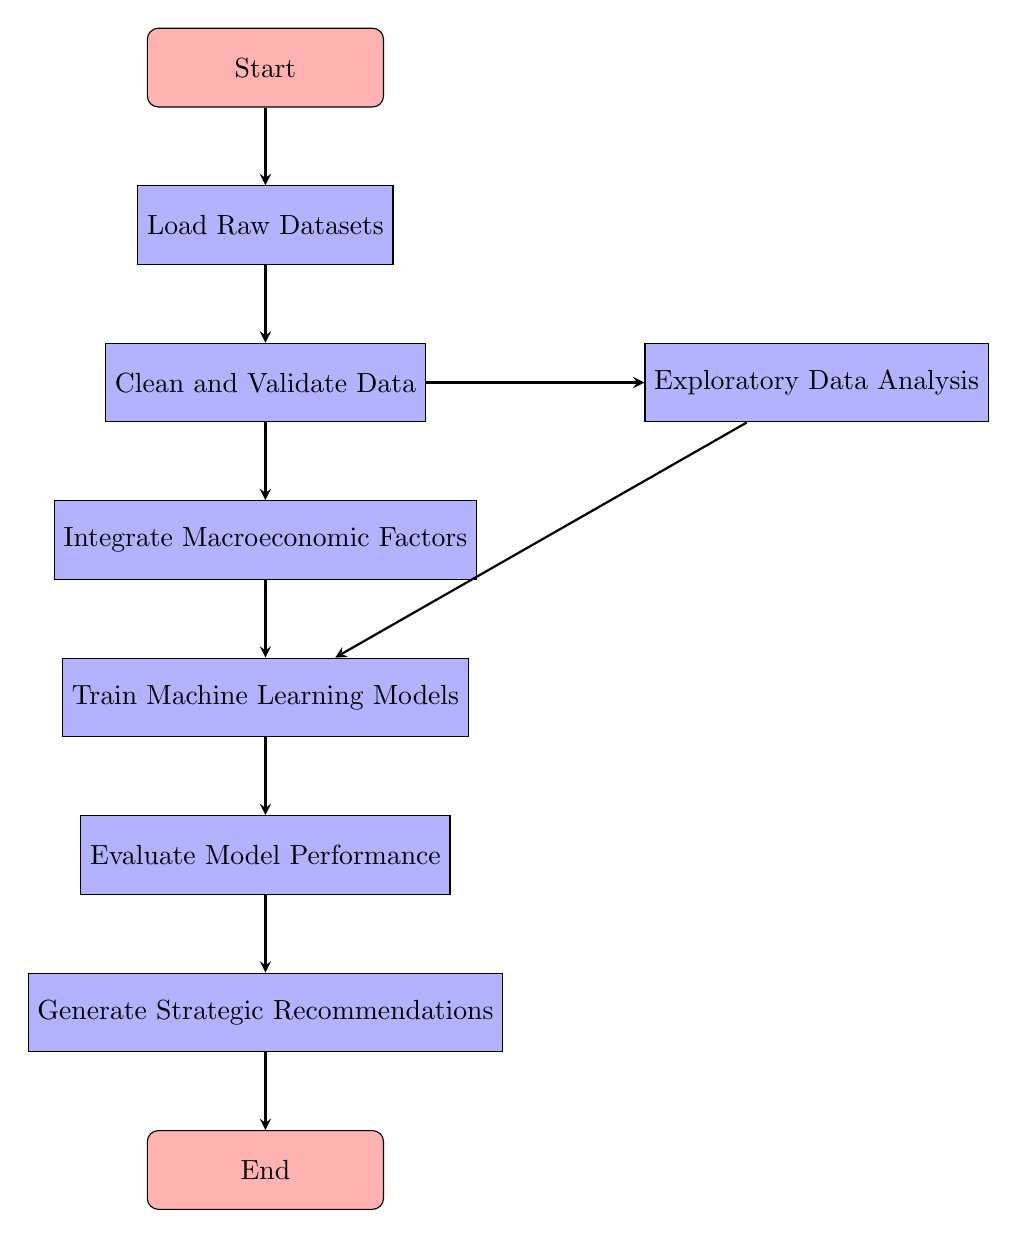
\begin{tikzpicture}[node distance=2cm]

\node (start) [startstop] {Start};
\node (load) [process, below of=start] {Load Raw Datasets};
\node (clean) [process, below of=load] {Clean and Validate Data};
\node (integrate) [process, below of=clean] {Integrate Macroeconomic Factors};
\node (eda) [process, right of=clean, xshift=5cm] {Exploratory Data Analysis};
\node (model) [process, below of=integrate] {Train Machine Learning Models};
\node (evaluate) [process, below of=model] {Evaluate Model Performance};
\node (recommend) [process, below of=evaluate] {Generate Strategic Recommendations};
\node (end) [startstop, below of=recommend] {End};

\draw [arrow] (start) -- (load);
\draw [arrow] (load) -- (clean);
\draw [arrow] (clean) -- (integrate);
\draw [arrow] (integrate) -- (model);
\draw [arrow] (model) -- (evaluate);
\draw [arrow] (evaluate) -- (recommend);
\draw [arrow] (recommend) -- (end);
\draw [arrow] (clean) -- (eda);
\draw [arrow] (eda) -- (model);

\end{tikzpicture}
\end{document}